%-------------------------------------------------------------------------------
% seq64_build
%-------------------------------------------------------------------------------
%
% \file        seq64_build.tex
% \library     Documents
% \author      Chris Ahlstrom
% \date        2015-11-06
% \update      2016-02-07
% \version     $Revision$
% \license     $XPC_GPL_LICENSE$
%
%     Provides the man page section of seq24-user-manual.tex.
%
%-------------------------------------------------------------------------------

\section{Building Sequencer64 From Source Code}
\label{sec:seq64_build}

   The current packaging for Sequencer64 is primarily aimed at developers.
   This section presents a bit of a how-to on building \textsl{Sequencer64}
   from source code.

\subsection{INSTALL}
\label{subsec:seq64_build_install}

   There are many build options.  Some of modifiable via the normal GNU
   \texttt{configure} script method.  Many more are modifiable by
   editing the source code to \textbf{define} and \textbf{undefine} certain
   macros.  If you don't care about options, start here.  If you want to
   see what options are available, skip to
   \sectionref{subsubsec:seq64_build_configure}, which has many details one can
   adjust.

   There is currently no \texttt{configure} script... it must be created
   by using the \texttt{bootstrap} script, as the following instructions make
   clear.

   \textbf{Steps:}

   \begin{enumber}
      \item Preload any DEPENDENCIES, as listed in the last section
         of this document.
          However, if some are missing, the configure script will tell you,
          or, at worst, a build error will tell you.
      \item Check-out the branch you want; normally you will be happy to
         get "master".  Make a branch if you want to make changes.
      \item From the top project directory, run the commands:
\begin{verbatim}
      $ ./bootstrap
      $ ./configure
\end{verbatim}
      \item For debugging without libtool getting in the way, just run
         one of the following commands, which will run the
         \texttt{configure} script, adding the
         \texttt{--enable-debug} and
         \texttt{--disable-shared} options to it.
\begin{verbatim}
      $ ./bootstrap --enable-debug
      $ ./bootstrap -ed
\end{verbatim}
      \item Run the make command:
\begin{verbatim}
      $ make
\end{verbatim}
      If you do not care about the documentation and debian packaging,
      change to the various sub-project directories before running make.
      \item To install \textsl{Sequencer64}, become root and run:
\begin{verbatim}
      # make install
\end{verbatim}
   \end{enumber}

   Please note that there are other things you can do to speed up the build
   process.  Already noted above is the \texttt{--enable-debug} option.
   The following command will bootstrap the code and then configure
   for release mode, and greatly reduce the amount of compiler output:
      
\begin{verbatim}
   $ ./bootstrap --enable-release
   $ ./bootstrap -er
\end{verbatim}

   This option will run the following command for you:

\begin{verbatim}
   $ ./configure --enable-silent-rules
\end{verbatim}

   This anti-verbosity option can be overridden at "make" time:

\begin{verbatim}
   $ make V=1
\end{verbatim}

   (Using \texttt{V=0} is another way to quiet down the build.)

   Also note that the build can be sped up by telling make to use more cores.
   For example, if you have an 8-core system:

\begin{verbatim}
   $ make -j 9
\end{verbatim}

   Of course, you can use fewer than the number of cores, if desired.

\subsection{Options for Sequencer64 Features}
\label{subsec:seq64_build_options}

   \textsl{Sequencer64} comes with options for the \texttt{configure} command
   and options represented by definable macros in the source code.

\subsubsection{Using More "configure" Options}
\label{subsubsec:seq64_build_configure}

   The following \texttt{configure} options can be specified on the command
   line:

   \setcounter{ItemCounter}{0}      % Reset the ItemCounter for this list.

   \itempar{\texttt{--disable-highlight}}{build!disable highlight}
        This option undefines the \texttt{SEQ64\_HIGHLIGHT\_EMPTY\_SEQS}
        macro, which is otherwise defined by default.  If defined, the
        application will
        highlight empty sequences/patterns by coloring them yellow.
        If not defined, empty sequences/patterns are shown in the normal
        black-on-white coloring.  In either case, empty patterns will not be
        played.

    \itempar{\texttt{--disable-lash}}{build!disable lash}
        This option undefines the \texttt{SEQ64\_LASH\_SUPPORT} macro, which is
        otherwise defined by default.  Even if this option is left defined,
        however, \textsl{Sequencer64} will still not use LASH support unless
        you specify \texttt{--lash} on the \texttt{sequencer64} command-line or
        turn on the new \texttt{[lash-session]} option in the "rc"
        configuration file,
        \texttt{~/.config/sequencer64/sequencer64.rc}.

    \itempar{\texttt{--disable-jack}}{build!disable jack}
        This option undefines the \texttt{SEQ64\_JACK\_SUPPORT} macro, which is
        otherwise defined by default.  Even if this option is left defined,
        however, \textsl{Sequencer64} will still not use JACK support unless
        you specify the various JACK options on the \texttt{sequencer64}
        command-line or turn them on in the "rc" configuration file,
        \texttt{~/.config/sequencer64/sequencer64.rc}.

    \itempar{\texttt{--disable-jack-session}}{build!disable jack session}
        This option undefines the \texttt{SEQ64\_JACK\_SESSION} macro, which is
        defined if JACK support is defined, and the jack/session.h file is
        found.  Again, this option, if left defined, can be affected by
        command-line options and options in the "rc" configuration file.

    To summarize, these options undefine the following build macros:

      \begin{itemize}
        \item \texttt{SEQ64\_HIGHLIGHT\_EMPTY\_SEQS}
        \item \texttt{SEQ64\_LASH\_SUPPORT}
        \item \texttt{SEQ64\_JACK\_SUPPORT}
        \item \texttt{SEQ64\_JACK\_SESSION}
      \end{itemize}

\subsubsection{Manually-defined Macros in the Code}
\label{subsubsec:seq64_build_macros}

   As we have explored what \textsl{Seq24} does while we add improvements to
   \textsl{Sequencer64}, we've found a lot of things that might change
   the code for the worse in some people's minds.  So we've been careful to
   mark those changes with macros.  And sometimes we tried a change, but left
   it disabled.

   You are free to look at those macros, modify them, and build the source code
   to your preferences.

   The following items are not yet part of the configure script, but can
   be edited manually to achieve the desired settings:

   \setcounter{ItemCounter}{0}      % Reset the ItemCounter for this list.
   
    \itempar{\texttt{SEQ64\_USE\_NEW\_FONT}}{build!new font}
        Already defined in the \texttt{font} module.
        If defined, a new, anti-aliased,
        bold font is used in the user-interface.  This new font is implemented
        in new XPM files in \texttt{resources/pixmaps} directory:
        \texttt{wen*.xpm}.  The font is slightly
        larger, but changes the user-interface sizes only to an infinitesmal
        degree.  Using this new font is the default.

        \textbf{Obsolete:}
        \index{obsolete:compile-time font}
        This option is no longer a compile-time option, but a run-time option.
        It is now the default, but the usage of the old versus new font can be
        set in the "user" configuration file.
        Also, if the legacy mode is specified, the old font becomes the
        default.

    \itempar{\texttt{SEQ64\_USE\_EVENT\_MAP}}{build!event map}
        Already defined in the \texttt{event\_list} module.
        It enables the usage of an
        \texttt{std::multimap}, instead of an \texttt{std::list},
        to store MIDI events.  Because
        the code does a lot of sorting of events, using the
        \texttt{std::multimap} is actually a lot faster (especially under debug
        mode, where it takes
        many seconds for a medium-size MIDI file to load using the
        \texttt{std::list} implementation.

        There is still a chance that the \texttt{std::multimap} might prove the
        limiting factor during playback.  If that is the case, then we would
        probably implement dumping the multimap to a vector before playback.
        We shall see!

    \itempar{\texttt{SEQ64\_USE\_MIDI\_VECTOR}}{build!midi vector}
        Already defined in the \texttt{midifile} module.
        It enables the usage of an
        \texttt{std::vector}, instead of an \texttt{std::list},
        to store MIDI data bytes.
        It provides the preferred alternative to the list for storing and
        counting the bytes of MIDI data.  It is an attempt to stop reversing
        certain events due to the peculiarities of using \texttt{std::list} to
        store MIDI bytes from a sequence.  This new implementation uses
        \texttt{std::vector} and does not use \texttt{pop\_back()} to retrieve
        the bytes for writing to a file.

   \textbf{Obsolete}:  Still need to replicate the descriptions that follow
      in the proper sections.

    \itempar{\texttt{SEQ64\_USE\_GREY\_GRID}}{build!grey/normal grid}
        \textbf{This item is no longer defined}.
        Instead, the option is now part of the "rc" configuration file.  This
        description will be moved to the correct section eventually.

        This configuration item causes the pattern slots/boxes to be colored
        grey (actually, they will be colored normally as per the current GTK
        them).  Otherwise, they are colored black.  By default, this value is
        defined (in the \texttt{mainwid} module).

    \itempar{\texttt{SEQ64\_USE\_WHITE\_GRID}}{build!white grid}
        \textbf{This item is no longer defined}.
        Instead, the option is now part of the "rc" configuration file.  This
        description will be moved to the correct section eventually.

        This configuration item causes the pattern slots/boxes to be colored
        white.  Also definable(in the \texttt{mainwid} module).

    \itempar{\texttt{SEQ64\_USE\_BRACKET\_GRID}}{build!normal grid}
        \textbf{This item is no longer defined}.
        Instead, the option is now part of the "rc" configuration file.  This
        description will be moved to the correct section eventually.

        This configuration box that outlines the pattern slots/boxes is
        painted over to convert the box to look like a pair of brackets.
        By default, this value is defined (in the \texttt{mainwid} module).

        Defining both of the macros (\texttt{USE\_GREY\_GRID} and
        \texttt{USE\_BRACKET\_GRID}) gives the normal Seq24 look for the Pattern
        Window.  Eventually we might move these definitions into the configure
        script, for easier
        modification.

    \itempar{\texttt{SEQ64\_SEQNUMBER\_ON\_GRID}}{build!grid numbers}
        \textbf{This item is no longer defined}.
        Instead, the option is now part of the "rc" configuration file.  This
        description will be moved to the correct section eventually.

        If the "show sequence numbers" option is on, then each
        of the blank pattern slots in the main window show the would-be
        sequence number for that slot.  The background color of the numbers
        will not match the background color of the grid (which matches the
        chosen GTK theme).  But, no matter what the GTK background color, they
        will at least be visible.  There is a little image of this style inside
        the screenshot shown on the first page of this manual.

        If \texttt{SEQ64\_USE\_WHITE\_GRID}
        are defined, so that the grid cells are white, then the sequence
        numbering looks a little nicer, as can be seen in the following
        figure:

\begin{figure}[H]
   \centering 
   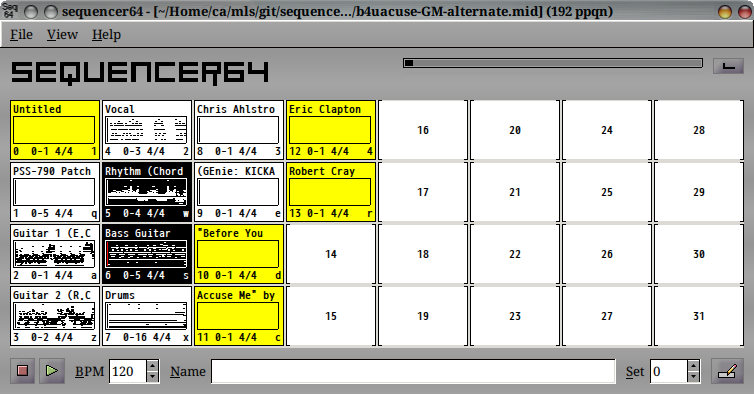
\includegraphics[scale=0.75]{pattern-window-white-box-numbering.png}
   \caption{Pattern Window Built for White Grid with Numbering}
   \label{fig:seq64_build_white_box_numbering}
\end{figure}

        There is a little image of this style inside the screenshot shown on
        the first page of this manual, as well.

        If neither \texttt{SEQ64\_USE\_GREY\_GRID} nor
        \texttt{SEQ64\_USE\_WHITE\_GRID} are defined, so that the grid slots
        are black, then the numbering will be yellow on a black background, and
        match perfectly.  This style is shown in the following figure:

\begin{figure}[H]
   \centering 
   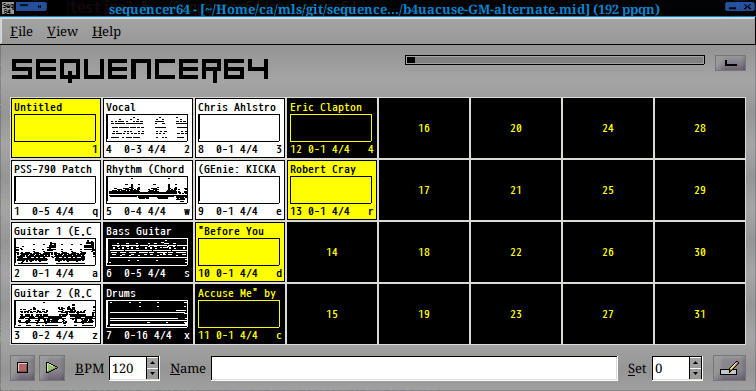
\includegraphics[scale=0.75]{pattern-window-black-box-numbering.png}
   \caption{Pattern Window Built for Black Grid with Numbering}
   \label{fig:seq64_build_black_box_numbering}
\end{figure}

      There is a little image of this style inside the screenshot shown on
      the first page of this manual, as well.

      Take your pick, modify the code accordingly before you build it.
      Perhaps these can eventually be options for the \texttt{configure}
      script, or even run-time options!  Let us know!

    \itempar{\texttt{SEQ64\_SOLID\_PIANOROLL\_GRID}}{build!solid piano-roll}
        Enabling this macro makes the grid lines for the piano rolls
        more solid, with about the same perception of lightness.
        It also calls in some other tweaks, such as the positioning of
        markers.  We currently like this look a little better, and so it is
        the default.  See the \texttt{app\_limits.h}
        header file for the definition of this variable.

        Here is the pattern editor (sequence editor) with this alternate look.

\begin{figure}[H]
   \centering 
   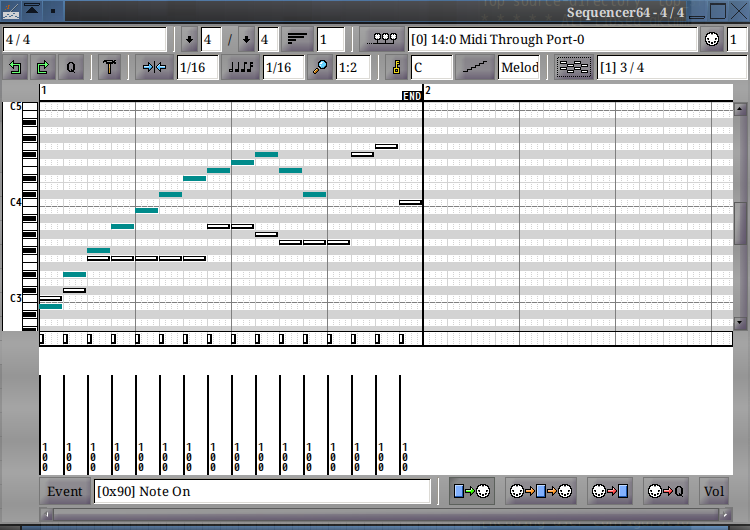
\includegraphics[scale=0.75]{pattern/pattern-editor-alternate-look.png}
   \caption{Sequence Pattern Editor Alternate Look}
   \label{fig:seq64_pattern_editor_alternate_look}
\end{figure}

        Note the smmoothness of the grid lines, the extra emphasis of the C
        notes at each octave, the emphasis of the note-drawing snap lines that
        mark the default length of a click-to-add note, the emphasis of the
        beat and bars, and, finally, the new location of the
        \textbf{END} marker.  Also note the dark-cyan background pattern,
        discussed elsewhere in this document.

        Here is the grid-styling for an 8/4 time signature in the song editor:

\begin{figure}[H]
   \centering 
   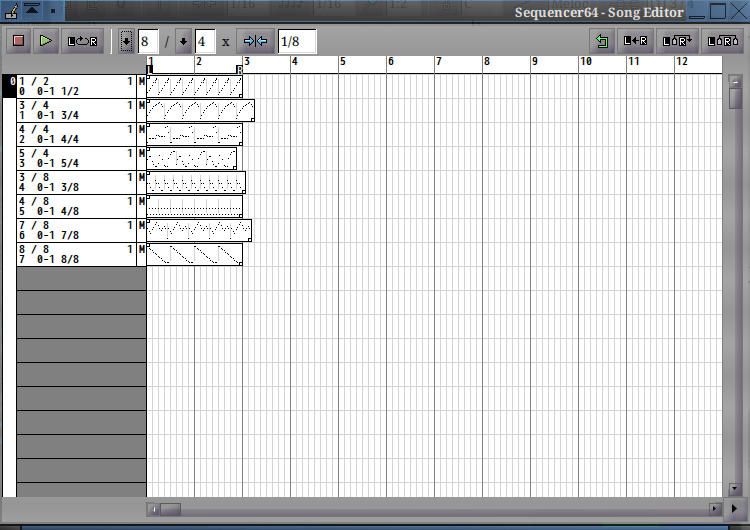
\includegraphics[scale=0.75]{song-editor/song-editor-alternate-look.png}
   \caption{Song Editor Alternate Look}
   \label{fig:seq64_song_editor_alternate_look}
\end{figure}

      Also note the sequence numbers shown in the bottom left of each pattern
      name box. This is a new feature, and, as noted elsewhere, is a new
      option in the \textsl{File / Options / Keyboard} tab and in
      the "rc" configuration file.

    \itempar{\texttt{SEQ64\_USE\_VI\_SEQROLL\_MODE}}{build!vi seqroll}
        Definable in the seqroll module, this macro allows the vi hjkl keys to
        be used as arrow keys for moving notes.  Not yet tested.  We will not
        make this a default, because it could drive non-vi users nuts.

    \itempar{\texttt{SEQ64\_USE\_DEBUG\_OUTPUT}}{build!debug output}
        Enable this macro in the globals.h header file, to see extra console
        output if the application is compiled for debugging.  This macro can be
        activated only if \texttt{PLATFORM\_DEBUG} is defined, which is taken
        care of by the build process.  If set, this macro turns on extra
        console output for the following modules:

        \begin{itemize}
           \item \texttt{globals}
           \item \texttt{jack\_assistant}
           \item \texttt{optionsfile}
           \item \texttt{user\_settings}
        \end{itemize}

    \itempar{\texttt{USE\_SEQ42\_PATCHES}}{build!seq42}
        This macro, in \texttt{globals.h}, currently merely marks a couple
        places where we found potentially useful code in the seq42 fork of
        seq24.

\subsection{Sequencer64 Build Dependencies}
\label{subsec:seq64_build_dependencies}

   With luck, the following dependencies will bring in their own
   dependencies when installed.

   Code:

     \begin{itemize}
        \item libgtkmm-2.4-dev (dev is the header-file package)
        \item libsigc++-2.0-dev
        \item libjack-jackd2-dev
        \item liblash-compat-dev (optional)
     \end{itemize}

   Runtime:

     \begin{itemize}
        \item libatk-adaptor (and its dependencies)
        \item libgail-common (and its dependencies)
        \item valgrind (optional, very useful for debugging)
        \item gdb (optional, very useful for debugging)
        \item gprof and gcov (optional, very useful for debugging)
     \end{itemize}

   Build tools:

     \begin{itemize}
        \item automake and autoconf
        \item autoconf-archive
        \item g++
        \item make
        \item libtool
        \item More?
     \end{itemize}

   Documentation:

     \begin{itemize}
        \item doxygen and doxygen-latex
        \item graphviz
        \item texlive
        \item More?
     \end{itemize}
      
   Debian packaging:

     \begin{itemize}
        \item debhelper
        \item fakeroot
        \item More?
     \end{itemize}

%-------------------------------------------------------------------------------
% vim: ts=3 sw=3 et ft=tex
%-------------------------------------------------------------------------------
